\chapter{Estudio de requisitos}
En este capítulo vamos a sentar las directrices del proyecto, utilizando la ingeniería de requisitos. Esto nos servirá de base para la implementación del sistema, además de marcar los límites de este y sus funcionalidades. 

\section{Actores}
Lo primero que se debe hacer a la hora de diseñar un sistema es encontrar las entidades con las que este se comunica, llamadas \textbf{actores}. 
En este caso existen dos: el conductor, que controla el vehículo, y la ECU, que maneja los subsistemas. Desde un punto de vista formal, podemos describirlos así: 


\begin{table}[H]
    \begin{tabular}{|llllll|}
    \hline
    \multicolumn{1}{|l|}{\textbf{Actor}}           & \multicolumn{4}{l|}{Conductor}                                                                                                                                                  & AC-01                 \\ \hline
    \multicolumn{1}{|l|}{\textbf{Descripción}}     & \multicolumn{5}{l|}{Es el conductor del vehículo.}                                                                                                                                                      \\ \hline
    \multicolumn{1}{|l|}{\textbf{Características}} & \multicolumn{5}{l|}{\begin{tabular}[c]{@{}l@{}}Tiene que mantener su atención centrada en la carretera, por lo que no\\  debe distraerse demasiado con complicaciones en los subsistemas.\end{tabular}} \\ \hline
    \multicolumn{1}{|l|}{\textbf{Relaciones}}      & \multicolumn{5}{l|}{Necesita la ECU para poder controlar el vehículo.}                                                                                                                                  \\ \hline
    \multicolumn{1}{|l|}{\textbf{Referencias}}     & \multicolumn{5}{l|}{CU-01 .. CU-08}                                                                                                                                                                     \\ \hline
    \multicolumn{1}{|l|}{\textbf{Autor}}           & \multicolumn{1}{l|}{Sheila Martínez}        & \multicolumn{1}{l|}{\textbf{Fecha}}        & \multicolumn{1}{l|}{25/06/2023}        & \multicolumn{1}{l|}{\textbf{Versión}}       & 1.0                   \\ \hline
    \multicolumn{6}{|l|}{\cellcolor[HTML]{DAE8FC}\textbf{Atributos}}                                                                                                                                                                                         \\ \hline
    \multicolumn{1}{|l|}{\textbf{Nombre}}          & \multicolumn{4}{l|}{\textbf{Descripción}}                                                                                                                                       & \textbf{Tipo}         \\ \hline
    \multicolumn{1}{|l|}{Alias}                    & \multicolumn{4}{l|}{\begin{tabular}[c]{@{}l@{}}Nombre que introduce el conductor \\ para ser identificado en el vehículo\end{tabular}}                                          & cadena de texto       \\ \hline
    \end{tabular}
    \end{table}

\begin{table}[H]
    \begin{tabular}{|llllll|}
    \hline
    \multicolumn{1}{|l|}{\textbf{Actor}}           & \multicolumn{4}{l|}{ECU}                                                                                                                                                                      & AC-02                   \\ \hline
    \multicolumn{1}{|l|}{\textbf{Descripción}}     & \multicolumn{5}{l|}{Es la unidad de control del vehículo.}                                                                                                                                                              \\ \hline
    \multicolumn{1}{|l|}{\textbf{Características}} & \multicolumn{5}{l|}{\begin{tabular}[c]{@{}l@{}}Controla todos los subsistemas del vehículo. Siempre debe tener \\ información actualizada de los valores de los sensores, y actuar\\ cuando sea necesario\end{tabular}} \\ \hline
    \multicolumn{1}{|l|}{\textbf{Relaciones}}      & \multicolumn{5}{l|}{Es controlada indirectamente por el conductor del vehículo}                                                                                                                                         \\ \hline
    \multicolumn{1}{|l|}{\textbf{Referencias}}     & \multicolumn{5}{l|}{CU-01 .. CU-17}                                                                                                                                                                                     \\ \hline
    \multicolumn{1}{|l|}{\textbf{Autor}}           & \multicolumn{1}{l|}{Sheila Martínez}            & \multicolumn{1}{l|}{\textbf{Fecha}}           & \multicolumn{1}{l|}{25/06/2023}           & \multicolumn{1}{l|}{\textbf{Versión}}           & 1.0                     \\ \hline
    \multicolumn{6}{|l|}{\cellcolor[HTML]{DAE8FC}\textbf{Atributos}}                                                                                                                                                                                                         \\ \hline
    \multicolumn{1}{|l|}{\textbf{Nombre}}          & \multicolumn{4}{l|}{\textbf{Descripción}}                                                                                                                                                     & \textbf{Tipo}           \\ \hline
    \multicolumn{1}{|l|}{}                         & \multicolumn{4}{l|}{}                                                                                                                                                                         &                         \\ \hline
    \end{tabular}
    \end{table}



    
\section{Casos de Uso}


Antes de comenzar a desarrollar el sistema, y una vez hemos descrito los actores, debemos asegurarnos de cuáles serán sus funcionalidades y sus características. Comenzaremos generando casos de uso, es decir, acciones (incluyendo variantes y/o errores), que un sistema puede realizar al interactuar con los actores. 

\begin{table}[H]
    \resizebox{\textwidth}{!}{%
    \begin{tabular}{|l|l|l|l|l|l|}
    \hline
    \textbf{Caso de Uso} & \multicolumn{3}{l|}{Encender motor} & \multicolumn{2}{l|}{CU-01} \\ \hline
    \textbf{Actores} & \multicolumn{5}{l|}{Conductor (I), ECU} \\ \hline
    \textbf{Tipo} & \multicolumn{5}{l|}{Primario, Esencial} \\ \hline
    \textbf{Referencias} & RF1 & \multicolumn{4}{l|}{CU-10} \\ \hline
    \textbf{Precondición} & \multicolumn{5}{l|}{El motor debe estar apagado} \\ \hline
    \textbf{Postcondición} & \multicolumn{5}{l|}{El motor se habrá encendido} \\ \hline
    \textbf{Autor} & Sheila Martínez & \textbf{Fecha} & 23/06/2023 & \textbf{Versión} & v.1 \\ \hline
    \multicolumn{6}{|l|}{\cellcolor[HTML]{ECF4FF}Propósito} \\ \hline
    \multicolumn{6}{|l|}{El conductor pulsa un botón, la ECU enciende el motor} \\ \hline
    \multicolumn{6}{|l|}{\cellcolor[HTML]{ECF4FF}Resumen} \\ \hline
    \multicolumn{6}{|l|}{\begin{tabular}[c]{@{}l@{}}1. El conductor pulsa el botón de arranque.\\  2. La ECU comprueba que el motor está apagado. \\ 3. La ECU arranca el motor.\end{tabular}} \\ \hline
    \end{tabular}%
    }
    \end{table}

    
\begin{table}[H]
    \resizebox{\textwidth}{!}{%
    \begin{tabular}{|l|l|l|l|l|l|}
    \hline
    \textbf{Caso de Uso} & \multicolumn{3}{l|}{Apagar motor} & \multicolumn{2}{l|}{CU-02} \\ \hline
    \textbf{Actores} & \multicolumn{5}{l|}{Conductor (I), ECU} \\ \hline
    \textbf{Tipo} & \multicolumn{5}{l|}{Primario, Esencial} \\ \hline
    \textbf{Referencias} & RF2 & \multicolumn{4}{l|}{CU-10} \\ \hline
    \textbf{Precondición} & \multicolumn{5}{l|}{El motor debe estar encendido} \\ \hline
    \textbf{Postcondición} & \multicolumn{5}{l|}{El motor se habrá apagado} \\ \hline
    \textbf{Autor} & Sheila Martínez & \textbf{Fecha} & 23/06/2023 & \textbf{Versión} & v.1 \\ \hline
    \multicolumn{6}{|l|}{\cellcolor[HTML]{ECF4FF}Propósito} \\ \hline
    \multicolumn{6}{|l|}{El conductor pulsa un botón, la ECU apaga el motor} \\ \hline
    \multicolumn{6}{|l|}{\cellcolor[HTML]{ECF4FF}Resumen} \\ \hline
    \multicolumn{6}{|l|}{\begin{tabular}[c]{@{}l@{}}1. El conductor pulsa el botón de apagado.\\  2. La ECU comprueba que el motor está encendido. \\ 3. La ECU apaga el motor.\end{tabular}} \\ \hline
    \end{tabular}%
    }
    \end{table}    


\begin{table}[H]
    \resizebox{\textwidth}{!}{%
    \begin{tabular}{|l|l|l|l|l|l|}
    \hline
    \textbf{Caso de Uso} & \multicolumn{3}{l|}{Encender luces} & \multicolumn{2}{l|}{CU-03} \\ \hline
    \textbf{Actores} & \multicolumn{5}{l|}{Conductor (I), ECU} \\ \hline
    \textbf{Tipo} & \multicolumn{5}{l|}{Primario, Esencial} \\ \hline
    \textbf{Referencias} & RF3 & \multicolumn{4}{l|}{CU-11} \\ \hline
    \textbf{Precondición} & \multicolumn{5}{l|}{Las luces deben estar apagadas} \\ \hline
    \textbf{Postcondición} & \multicolumn{5}{l|}{Las luces se habrán encendido} \\ \hline
    \textbf{Autor} & Sheila Martínez & \textbf{Fecha} & 23/06/2023 & \textbf{Versión} & v.1 \\ \hline
    \multicolumn{6}{|l|}{\cellcolor[HTML]{ECF4FF}Propósito} \\ \hline
    \multicolumn{6}{|l|}{El conductor pulsa un botón, la ECU enciende las luces} \\ \hline
    \multicolumn{6}{|l|}{\cellcolor[HTML]{ECF4FF}Resumen} \\ \hline
    \multicolumn{6}{|l|}{\begin{tabular}[c]{@{}l@{}}1. El conductor pulsa el botón de encendido de luces.\\  2. La ECU comprueba que las luces están apagadas. \\ 3. La ECU enciende las luces \\ 4. La ECU enciende el piloto que indica que las luces están encendidas.\end{tabular}} \\ \hline
    \end{tabular}%
    }
\end{table}


\begin{table}[H]
    \resizebox{\textwidth}{!}{%
    \begin{tabular}{|l|l|l|l|l|l|}
    \hline
    \textbf{Caso de Uso} & \multicolumn{3}{l|}{Apagar luces} & \multicolumn{2}{l|}{CU-04} \\ \hline
    \textbf{Actores} & \multicolumn{5}{l|}{Conductor (I), ECU} \\ \hline
    \textbf{Tipo} & \multicolumn{5}{l|}{Primario, Esencial} \\ \hline
    \textbf{Referencias} & RF3 & \multicolumn{4}{l|}{CU-11} \\ \hline
    \textbf{Precondición} & \multicolumn{5}{l|}{Las luces deben estar encendidas} \\ \hline
    \textbf{Postcondición} & \multicolumn{5}{l|}{Las luces se habrán apagado} \\ \hline
    \textbf{Autor} & Sheila Martínez & \textbf{Fecha} & 23/06/2023 & \textbf{Versión} & v.1 \\ \hline
    \multicolumn{6}{|l|}{\cellcolor[HTML]{ECF4FF}Propósito} \\ \hline
    \multicolumn{6}{|l|}{El conductor pulsa un botón, la ECU apaga las luces} \\ \hline
    \multicolumn{6}{|l|}{\cellcolor[HTML]{ECF4FF}Resumen} \\ \hline
    \multicolumn{6}{|l|}{\begin{tabular}[c]{@{}l@{}}1. El conductor pulsa el botón de apagado de luces.\\ 2. La ECU comprueba que las luces están encendidas.\\ 3. La ECU apaga las luces.\end{tabular}} \\ \hline
    \end{tabular}%
    }
    \end{table}

\begin{table}[H]
    \resizebox{\textwidth}{!}{%
    \begin{tabular}{|l|l|l|l|l|l|}
    \hline
    \textbf{Caso de Uso} & \multicolumn{3}{l|}{Encender intermitente} & \multicolumn{2}{l|}{CU-05} \\ \hline
    \textbf{Actores} & \multicolumn{5}{l|}{Conductor (I), ECU} \\ \hline
    \textbf{Tipo} & \multicolumn{5}{l|}{Primario, Esencial} \\ \hline
    \textbf{Referencias} & RF5 & \multicolumn{4}{l|}{CU-11} \\ \hline
    \textbf{Precondición} & \multicolumn{5}{l|}{Los intermitentes deben estar apagados} \\ \hline
    \textbf{Postcondición} & \multicolumn{5}{l|}{Se habrá accionado el intermitente de la dirección deseada} \\ \hline
    \textbf{Autor} & Sheila Martínez & \textbf{Fecha} & 23/06/2023 & \textbf{Versión} & v.1 \\ \hline
    \multicolumn{6}{|l|}{\cellcolor[HTML]{ECF4FF}Propósito} \\ \hline
    \multicolumn{6}{|l|}{El conductor acciona una palanca, la ECU enciende la luz intermitente} \\ \hline
    \multicolumn{6}{|l|}{\cellcolor[HTML]{ECF4FF}Resumen} \\ \hline
    \multicolumn{6}{|l|}{\begin{tabular}[c]{@{}l@{}}1. El conductor acciona la palanca hacia el lado deseado\\ 2. La ECU comprueba que el intermitente no está accionado\\ 3. La ECU enciende el intermitente de ese lado\end{tabular}} \\ \hline
    \end{tabular}%
    }
    \end{table}

\begin{table}[H]
    \resizebox{\textwidth}{!}{%
    \begin{tabular}{|l|l|l|l|l|l|}
    \hline
    \textbf{Caso de Uso} & \multicolumn{3}{l|}{Apagar intermitente} & \multicolumn{2}{l|}{CU-06} \\ \hline
    \textbf{Actores} & \multicolumn{5}{l|}{Conductor (I), ECU} \\ \hline
    \textbf{Tipo} & \multicolumn{5}{l|}{Primario, Esencial} \\ \hline
    \textbf{Referencias} & RF6 & \multicolumn{4}{l|}{CU-11} \\ \hline
    \textbf{Precondición} & \multicolumn{5}{l|}{El intermitente debe estar accionado hacia uno de los dos lados} \\ \hline
    \textbf{Postcondición} & \multicolumn{5}{l|}{Se habrán apagado los intermitentes} \\ \hline
    \textbf{Autor} & Sheila Martínez & \textbf{Fecha} & 23/06/2023 & \textbf{Versión} & v.1 \\ \hline
    \multicolumn{6}{|l|}{\cellcolor[HTML]{ECF4FF}Propósito} \\ \hline
    \multicolumn{6}{|l|}{El conductor devuelve una palanca a su estado inicial, la ECU apaga la luz intermitente} \\ \hline
    \multicolumn{6}{|l|}{\cellcolor[HTML]{ECF4FF}Resumen} \\ \hline
    \multicolumn{6}{|l|}{\begin{tabular}[c]{@{}l@{}}1. El conductor devuelve la palanca hacia su estado inicial\\ 2. La ECU apaga los intermitentes\end{tabular}} \\ \hline
    \end{tabular}%
    }
\end{table}

\begin{table}[H]
    \resizebox{\textwidth}{!}{%
    \begin{tabular}{|l|l|l|l|l|l|}
    \hline
    \textbf{Caso de Uso} & \multicolumn{3}{l|}{Cambiar estado luz freno} & \multicolumn{2}{l|}{CU-07} \\ \hline
    \textbf{Actores} & \multicolumn{5}{l|}{Conductor (I), ECU} \\ \hline
    \textbf{Tipo} & \multicolumn{5}{l|}{Primario, Esencial} \\ \hline
    \textbf{Referencias} & RF7 & \multicolumn{4}{l|}{CU-11} \\ \hline
    \textbf{Precondición} & \multicolumn{5}{l|}{} \\ \hline
    \textbf{Postcondición} & \multicolumn{5}{l|}{Se habrá encendido la luz de freno} \\ \hline
    \textbf{Autor} & Sheila Martínez & \textbf{Fecha} & 23/06/2023 & \textbf{Versión} & v.1 \\ \hline
    \multicolumn{6}{|l|}{\cellcolor[HTML]{ECF4FF}Propósito} \\ \hline
    \multicolumn{6}{|l|}{El conductor pisa el pedal de freno, se enciende la luz de freno} \\ \hline
    \multicolumn{6}{|l|}{\cellcolor[HTML]{ECF4FF}Resumen} \\ \hline
    \multicolumn{6}{|l|}{\begin{tabular}[c]{@{}l@{}}1. El conductor pisa el pedal de freno\\ 2. La ECU detecta que el freno ha sido pulsado\\ 3. La ECU enciende la luz de freno\\ 3.1 El conductor suelta el pedal de freno\\ 3.2 La ECU detecta que el freno ha sido soltado\\ 3.3 La ECU apaga la luz de freno\end{tabular}} \\ \hline
    \end{tabular}%
    }
\end{table}


\begin{table}[H]
    \resizebox{\textwidth}{!}{%
    \begin{tabular}{|l|l|l|l|l|l|}
    \hline
    \textbf{Caso de Uso} & \multicolumn{3}{l|}{Cambiar velocidad} & \multicolumn{2}{l|}{CU-08} \\ \hline
    \textbf{Actores} & \multicolumn{5}{l|}{Conductor (I), ECU} \\ \hline
    \textbf{Tipo} & \multicolumn{5}{l|}{Primario, Esencial} \\ \hline
    \textbf{Referencias} & RF8 & \multicolumn{4}{l|}{-} \\ \hline
    \textbf{Precondición} & \multicolumn{5}{l|}{El motor debe estar encendido} \\ \hline
    \textbf{Postcondición} & \multicolumn{5}{l|}{Se habrá variado la velocidad} \\ \hline
    \textbf{Autor} & Sheila Martínez & \textbf{Fecha} & 23/06/2023 & \textbf{Versión} & v.1 \\ \hline
    \multicolumn{6}{|l|}{\cellcolor[HTML]{ECF4FF}Propósito} \\ \hline
    \multicolumn{6}{|l|}{El conductor pisa el pedal de acelerador, el motor acelera proporcionalmente} \\ \hline
    \multicolumn{6}{|l|}{\cellcolor[HTML]{ECF4FF}Resumen} \\ \hline
    \multicolumn{6}{|l|}{\begin{tabular}[c]{@{}l@{}}1. El conductor pisa el acelerador\\ 2. La ECU detecta que ha sido pulsado y con cuánta intensidad.\\ 3. La ECU varía la velocidad en función de la intensidad.\end{tabular}} \\ \hline
    \end{tabular}%
    }
    \end{table}


\begin{table}[H]
    \resizebox{\textwidth}{!}{%
    \begin{tabular}{|l|l|l|l|l|l|}
    \hline
    \textbf{Caso de Uso} & \multicolumn{3}{l|}{Comprobar temperatura motor} & \multicolumn{2}{l|}{CU-09} \\ \hline
    \textbf{Actores} & \multicolumn{5}{l|}{ECU} \\ \hline
    \textbf{Tipo} & \multicolumn{5}{l|}{Primario, Esencial} \\ \hline
    \textbf{Referencias} & RF9 & \multicolumn{4}{l|}{CU-17} \\ \hline
    \textbf{Precondición} & \multicolumn{5}{l|}{} \\ \hline
    \textbf{Postcondición} & \multicolumn{5}{l|}{Se habrá leído y comprobado el valor de la temperatura del motor} \\ \hline
    \textbf{Autor} & Sheila Martínez & \textbf{Fecha} & 23/06/2023 & \textbf{Versión} & v.1 \\ \hline
    \multicolumn{6}{|l|}{\cellcolor[HTML]{ECF4FF}Propósito} \\ \hline
    \multicolumn{6}{|l|}{La ECU obtiene el valor de la temperatura del motor y comprueba si es correcta.} \\ \hline
    \multicolumn{6}{|l|}{\cellcolor[HTML]{ECF4FF}Resumen} \\ \hline
    \multicolumn{6}{|l|}{\begin{tabular}[c]{@{}l@{}}1. La ECU obtiene el valor de la temperatura del motor.\\ 2. Comprueba si el valor es correcto.\\ \\ 2.1 Si es incorrecto, enciende un piloto que lo indica.\end{tabular}} \\ \hline
    \end{tabular}%
    }
    \end{table}

    \begin{table}[H]
        \resizebox{\textwidth}{!}{%
        \begin{tabular}{|l|l|l|l|l|l|}
        \hline
        \textbf{Caso de Uso} & \multicolumn{3}{l|}{Comprobar estado motor} & \multicolumn{2}{l|}{CU-10} \\ \hline
        \textbf{Actores} & \multicolumn{5}{l|}{ECU} \\ \hline
        \textbf{Tipo} & \multicolumn{5}{l|}{Primario, Esencial} \\ \hline
        \textbf{Referencias} & RF9 & \multicolumn{4}{l|}{-} \\ \hline
        \textbf{Precondición} & \multicolumn{5}{l|}{} \\ \hline
        \textbf{Postcondición} & \multicolumn{5}{l|}{Se habrá leído y comprobado el estado del motor} \\ \hline
        \textbf{Autor} & Sheila Martínez & \textbf{Fecha} & 23/06/2023 & \textbf{Versión} & v.1 \\ \hline
        \multicolumn{6}{|l|}{\cellcolor[HTML]{ECF4FF}Propósito} \\ \hline
        \multicolumn{6}{|l|}{La ECU obtiene el estado del motor} \\ \hline
        \multicolumn{6}{|l|}{\cellcolor[HTML]{ECF4FF}Resumen} \\ \hline
        \multicolumn{6}{|l|}{\begin{tabular}[c]{@{}l@{}}1. La ECU obtiene el estado del motor \end{tabular}} \\ \hline
        \end{tabular}%
        }
        \end{table}


\begin{table}[H]
    \resizebox{\textwidth}{!}{%
    \begin{tabular}{|l|l|l|l|l|l|}
    \hline
    \textbf{Caso de Uso} & \multicolumn{3}{l|}{Comprobar estado luces} & \multicolumn{2}{l|}{CU-11} \\ \hline
    \textbf{Actores} & \multicolumn{5}{l|}{ECU} \\ \hline
    \textbf{Tipo} & \multicolumn{5}{l|}{Primario, Esencial} \\ \hline
    \textbf{Referencias} & RF9 & \multicolumn{4}{l|}{-} \\ \hline
    \textbf{Precondición} & \multicolumn{5}{l|}{} \\ \hline
    \textbf{Postcondición} & \multicolumn{5}{l|}{Se habrá leído y comprobado el estado de las luces} \\ \hline
    \textbf{Autor} & Sheila Martínez & \textbf{Fecha} & 23/06/2023 & \textbf{Versión} & v.1 \\ \hline
    \multicolumn{6}{|l|}{\cellcolor[HTML]{ECF4FF}Propósito} \\ \hline
    \multicolumn{6}{|l|}{La ECU obtiene el estado de las luces} \\ \hline
    \multicolumn{6}{|l|}{\cellcolor[HTML]{ECF4FF}Resumen} \\ \hline
    \multicolumn{6}{|l|}{1. La ECU obtiene el estado de las luces} \\ \hline
    \end{tabular}%
    }
    \end{table}


    \begin{table}[H]
        \resizebox{\textwidth}{!}{%
        \begin{tabular}{|l|l|l|l|l|l|}
        \hline
        \textbf{Caso de Uso} & \multicolumn{3}{l|}{Comprobar temperatura batería} & \multicolumn{2}{l|}{CU-12} \\ \hline
        \textbf{Actores} & \multicolumn{5}{l|}{ECU} \\ \hline
        \textbf{Tipo} & \multicolumn{5}{l|}{Primario, Esencial} \\ \hline
        \textbf{Referencias} & RF9 & \multicolumn{4}{l|}{CU-17} \\ \hline
        \textbf{Precondición} & \multicolumn{5}{l|}{} \\ \hline
        \textbf{Postcondición} & \multicolumn{5}{l|}{Se habrá leído y comprobado el valor de la temperatura de la batería} \\ \hline
        \textbf{Autor} & Sheila Martínez & \textbf{Fecha} & 23/06/2023 & \textbf{Versión} & v.1 \\ \hline
        \multicolumn{6}{|l|}{\cellcolor[HTML]{ECF4FF}Propósito} \\ \hline
        \multicolumn{6}{|l|}{La ECU obtiene el valor de la temperatura de la batería y comprueba si es correcta.} \\ \hline
        \multicolumn{6}{|l|}{\cellcolor[HTML]{ECF4FF}Resumen} \\ \hline
        \multicolumn{6}{|l|}{\begin{tabular}[c]{@{}l@{}}1. La ECU obtiene el valor de la temperatura de la batería.\\ 2. Comprueba si el valor es correcto.\\ \\ 2.1 Si es incorrecto, enciende un piloto que lo indica.\end{tabular}} \\ \hline
        \end{tabular}%
        }
        \end{table}


        \begin{table}[H]
            \resizebox{\textwidth}{!}{%
            \begin{tabular}{|l|l|l|l|l|l|}
            \hline
            \textbf{Caso de Uso} & \multicolumn{3}{l|}{Leer voltaje sistema} & \multicolumn{2}{l|}{CU-13} \\ \hline
            \textbf{Actores} & \multicolumn{5}{l|}{ECU} \\ \hline
            \textbf{Tipo} & \multicolumn{5}{l|}{Primario, Real} \\ \hline
            \textbf{Referencias} & RF9 & \multicolumn{4}{l|}{-} \\ \hline
            \textbf{Precondición} & \multicolumn{5}{l|}{} \\ \hline
            \textbf{Postcondición} & \multicolumn{5}{l|}{Se habrá leído y comprobado el voltaje} \\ \hline
            \textbf{Autor} & Sheila Martínez & \textbf{Fecha} & 23/06/2023 & \textbf{Versión} & v.1 \\ \hline
            \multicolumn{6}{|l|}{\cellcolor[HTML]{ECF4FF}Propósito} \\ \hline
            \multicolumn{6}{|l|}{La ECU obtiene el voltaje del sistema} \\ \hline
            \multicolumn{6}{|l|}{\cellcolor[HTML]{ECF4FF}Resumen} \\ \hline
            \multicolumn{6}{|l|}{1. La ECU obtiene el voltaje del sistema} \\ \hline
            \end{tabular}%
            }
            \end{table}


\begin{table}[H]
    \resizebox{\textwidth}{!}{%
    \begin{tabular}{|l|l|l|l|l|l|}
    \hline
    \textbf{Caso de Uso} & \multicolumn{3}{l|}{Calcular consumo} & \multicolumn{2}{l|}{CU-14} \\ \hline
    \textbf{Actores} & \multicolumn{5}{l|}{ECU} \\ \hline
    \textbf{Tipo} & \multicolumn{5}{l|}{Primario, Esencial} \\ \hline
    \textbf{Referencias} & RF9 & \multicolumn{4}{l|}{CU-13} \\ \hline
    \textbf{Precondición} & \multicolumn{5}{l|}{Se debe haber leído el voltaje de la batería} \\ \hline
    \textbf{Postcondición} & \multicolumn{5}{l|}{Se habrá calculado el consumo} \\ \hline
    \textbf{Autor} & Sheila Martínez & \textbf{Fecha} & 23/06/2023 & \textbf{Versión} & v.1 \\ \hline
    \multicolumn{6}{|l|}{\cellcolor[HTML]{ECF4FF}Propósito} \\ \hline
    \multicolumn{6}{|l|}{La ECU obtiene el consumo instantáneo} \\ \hline
    \multicolumn{6}{|l|}{\cellcolor[HTML]{ECF4FF}Resumen} \\ \hline
    \multicolumn{6}{|l|}{1. La ECU obtiene el consumo instantáneo} \\ \hline
    \end{tabular}%
    }
    \end{table}

\begin{table}[H]
    \resizebox{\textwidth}{!}{%
    \begin{tabular}{|l|l|l|l|l|l|}
    \hline
    \textbf{Caso de Uso} & \multicolumn{3}{l|}{Calcular autonomía} & \multicolumn{2}{l|}{CU-15} \\ \hline
    \textbf{Actores} & \multicolumn{5}{l|}{ECU} \\ \hline
    \textbf{Tipo} & \multicolumn{5}{l|}{Primario, Esencial} \\ \hline
    \textbf{Referencias} & RF9 & \multicolumn{4}{l|}{CU-14} \\ \hline
    \textbf{Precondición} & \multicolumn{5}{l|}{Se debe saber el voltaje máximo de la batería y el consumo} \\ \hline
    \textbf{Postcondición} & \multicolumn{5}{l|}{Se habrá calculado la autonomía} \\ \hline
    \textbf{Autor} & Sheila Martínez & \textbf{Fecha} & 23/06/2023 & \textbf{Versión} & v.1 \\ \hline
    \multicolumn{6}{|l|}{\cellcolor[HTML]{ECF4FF}Propósito} \\ \hline
    \multicolumn{6}{|l|}{La ECU obtiene la autonomía del sistema} \\ \hline
    \multicolumn{6}{|l|}{\cellcolor[HTML]{ECF4FF}Resumen} \\ \hline
    \multicolumn{6}{|l|}{La ECU obtiene la autonomía del sistema en tiempo y porcentaje} \\ \hline
    \end{tabular}%
    }
    \end{table}


\begin{table}[H]
    \resizebox{\textwidth}{!}{%
    \begin{tabular}{|l|l|l|l|l|l|}
    \hline
    \textbf{Caso de Uso} & \multicolumn{3}{l|}{Calcular carga batería} & \multicolumn{2}{l|}{CU-16} \\ \hline
    \textbf{Actores} & \multicolumn{5}{l|}{ECU} \\ \hline
    \textbf{Tipo} & \multicolumn{5}{l|}{Primario, Esencial} \\ \hline
    \textbf{Referencias} & RF9 & \multicolumn{4}{l|}{CU-13} \\ \hline
    \textbf{Precondición} & \multicolumn{5}{l|}{Se debe saber el voltaje máximo de la batería y el voltaje actual} \\ \hline
    \textbf{Postcondición} & \multicolumn{5}{l|}{Se habrá calculado la carga de la batería} \\ \hline
    \textbf{Autor} & Sheila Martínez & \textbf{Fecha} & 23/06/2023 & \textbf{Versión} & v.1 \\ \hline
    \multicolumn{6}{|l|}{\cellcolor[HTML]{ECF4FF}Propósito} \\ \hline
    \multicolumn{6}{|l|}{La ECU obtiene la carga de la batería} \\ \hline
    \multicolumn{6}{|l|}{\cellcolor[HTML]{ECF4FF}Resumen} \\ \hline
    \multicolumn{6}{|l|}{La ECU obtiene la carga de la batería en porcentaje} \\ \hline
    \end{tabular}%
    }
    \end{table}

%    \begin{table}[]
%        \resizebox{\textwidth}{!}{%
%        \begin{tabular}{|l|l|l|l|l|l|}
%        \hline
%        \textbf{Caso de Uso} & \multicolumn{3}{l|}{Variar voltaje} & \multicolumn{2}{l|}{CU-16} \\ \hline
%        \textbf{Actores} & \multicolumn{5}{l|}{ECU} \\ \hline
%        \textbf{Tipo} & \multicolumn{5}{l|}{Primario, Esencial} \\ \hline
%        \textbf{Referencias} & Requisitos que se pueden incluir dentro de este cu & \multicolumn{4}{l|}{Cu que tiene relacion} \\ \hline
%        \textbf{Precondición} & \multicolumn{5}{l|}{Se debe tener un valor al que variar el voltaje} \\ \hline
%        \textbf{Postcondición} & \multicolumn{5}{l|}{Se habrá variado el voltaje} \\ \hline
%        \textbf{Autor} & Sheila Martínez & \textbf{Fecha} & 23/06/2023 & \textbf{Versión} & v.1 \\ \hline
%        \multicolumn{6}{|l|}{\cellcolor[HTML]{ECF4FF}Propósito} \\ \hline
%        \multicolumn{6}{|l|}{La ECU varía el voltaje en relación al valor recibido} \\ \hline
%        \multicolumn{6}{|l|}{\cellcolor[HTML]{ECF4FF}Resumen} \\ \hline
%        \multicolumn{6}{|l|}{La ECU varía el voltaje del sistema conforme al valor que se le ha dado, tras comprobar que este valor es correcto.} \\ \hline
%        \end{tabular}%
%        }
%       \end{table}


\begin{table}[H]
    \resizebox{\textwidth}{!}{%
    \begin{tabular}{|l|l|l|l|l|l|}
    \hline
    \textbf{Caso de Uso} & \multicolumn{3}{l|}{Mostrar datos} & \multicolumn{2}{l|}{CU-17} \\ \hline
    \textbf{Actores} & \multicolumn{5}{l|}{ECU} \\ \hline
    \textbf{Tipo} & \multicolumn{5}{l|}{Primario, Esencial} \\ \hline
    \textbf{Referencias} & RF9 & \multicolumn{4}{l|}{-} \\ \hline
    \textbf{Precondición} & \multicolumn{5}{l|}{Se deben tener calculados y leídos todos los datos del sistema} \\ \hline
    \textbf{Postcondición} & \multicolumn{5}{l|}{Se mostrarán los datos del sistema} \\ \hline
    \textbf{Autor} & Sheila Martínez & \textbf{Fecha} & 23/06/2023 & \textbf{Versión} & v.1 \\ \hline
    \multicolumn{6}{|l|}{\cellcolor[HTML]{ECF4FF}Propósito} \\ \hline
    \multicolumn{6}{|l|}{La ECU muestra los datos del sistema} \\ \hline
    \multicolumn{6}{|l|}{\cellcolor[HTML]{ECF4FF}Resumen} \\ \hline
    \multicolumn{6}{|l|}{\begin{tabular}[c]{@{}l@{}}La ECU muestra por pantalla todos los datos obtenidos por los sensores\\  para que el conductor pueda servirse de ellos\end{tabular}} \\ \hline
    \end{tabular}%
    }
\end{table}

\newpage
\section{Diagramas de casos de uso}

Una vez realizados los casos de uso, los \textbf{diagramas de uso} nos permiten tener una visión general del conjunto de subsistemas, así como su interacción con los actores: 


\begin{figure}[H]
    \centering
    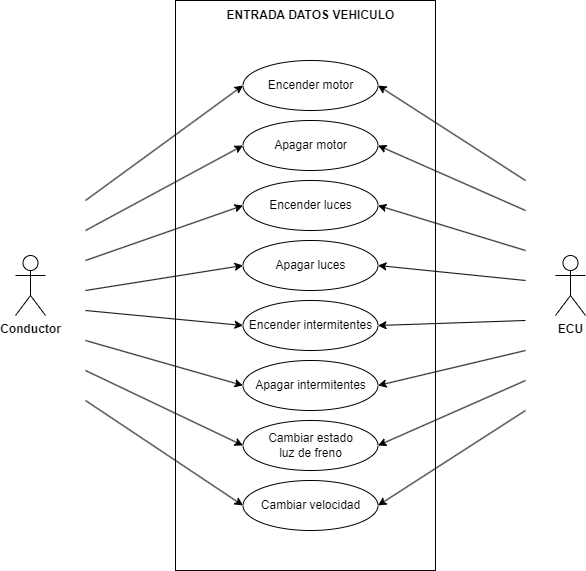
\includegraphics[width=1.1\textwidth]{imagenes/diagrama_CU_1.png}
\end{figure}

\begin{figure}[H]
    \centering
    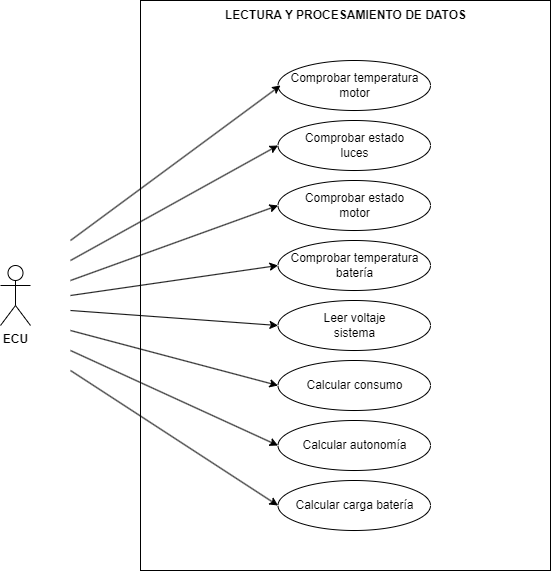
\includegraphics[width=1\textwidth]{imagenes/diagrama_CU_2.png}
\end{figure}

\begin{figure}[H]
    \centering
    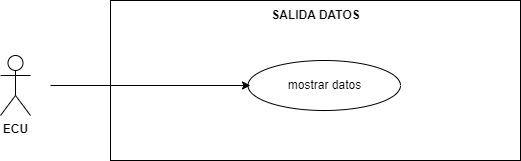
\includegraphics[width=1\textwidth]{imagenes/diagrama_CU_3.png}
\end{figure}


\section{Requisitos}

Los requisitos nos van a permitir comprender y designar cuáles serán las capacidades y funciones de nuestro producto para resolver una necesidad expresada por el usuario. Existen dos tipos principales, que se exponen a continuación.

\subsection*{Requisitos funcionales}

Los requisitos funcionales son aquellos requisitos que describen las funciones que debe realizar el sistema, es decir, la interacción entre este y su entorno, e indican cuál debe ser la reacción al sistema ante una determinada entrada. 

\begin{table}[H]
    \resizebox{\textwidth}{!}{%
    \begin{tabular}{|l|l|}
    \hline
    \textbf{Nº de RF} & 1 \\ \hline
    \textbf{Nombre} & Encender el motor \\ \hline
    \textbf{Descripción} & Como conductor, quiero poder encender el motor del vehículo \\ \hline
    \textbf{Prioridad} & Alta \\ \hline
    \textbf{Entrada} & Una señal \\ \hline
    \textbf{Prerrequisitos} & El motor debe estar apagado \\ \hline
    \textbf{Procesamiento} & El usuario pulsa el botón de arranque y el motor se activa \\ \hline
    \rowcolor[HTML]{FFFFFF} 
    \textbf{Postcondición} & - \\ \hline
    \end{tabular}%
    }
    \end{table}

\begin{table}[H]
    \resizebox{\textwidth}{!}{%
    \begin{tabular}{|l|l|}
    \hline
    \textbf{Nº de RF} & 2 \\ \hline
    \textbf{Nombre} & Apagar el motor \\ \hline
    \textbf{Descripción} & Como conductor, quiero poder apagar el motor del vehículo \\ \hline
    \textbf{Prioridad} & Alta \\ \hline
    \textbf{Entrada} & Una señal \\ \hline
    \textbf{Prerrequisitos} & El motor debe estar encendido \\ \hline
    \textbf{Procesamiento} & El usuario pulsa el botón de arranque y el motor se apaga \\ \hline
    \rowcolor[HTML]{FFFFFF} 
    \textbf{Postcondición} & - \\ \hline
    \end{tabular}%
    }
    \end{table}


\begin{table}[H]
    \resizebox{\textwidth}{!}{%
    \begin{tabular}{|l|l|}
    \hline
    \textbf{Nº de RF} & 3 \\ \hline
    \textbf{Nombre} & Encender las luces \\ \hline
    \textbf{Descripción} & Como conductor, quiero poder encender las luces del vehículo \\ \hline
    \textbf{Prioridad} & Media \\ \hline
    \textbf{Entrada} & Una señal \\ \hline
    \textbf{Prerrequisitos} & Las luces deben estar apagadas \\ \hline
    \textbf{Procesamiento} & El usuario pulsa el botón de encendido de luces y las luces se encienden \\ \hline
    \rowcolor[HTML]{FFFFFF} 
    \textbf{Postcondición} & - \\ \hline
    \end{tabular}%
    }
    \end{table}


\begin{table}[H]
    \resizebox{\textwidth}{!}{%
    \begin{tabular}{|l|l|}
    \hline
    \textbf{Nº de RF} & 4 \\ \hline
    \textbf{Nombre} & Apagar las luces \\ \hline
    \textbf{Descripción} & Como conductor, quiero poder apagar las luces del vehículo \\ \hline
    \textbf{Prioridad} & Media \\ \hline
    \textbf{Entrada} & Una señal \\ \hline
    \textbf{Prerrequisitos} & Las luces deben estar encendidas \\ \hline
    \textbf{Procesamiento} & El usuario pulsa el botón de apagado de luces y las luces se apagan \\ \hline
    \rowcolor[HTML]{FFFFFF} 
    \textbf{Postcondición} & - \\ \hline
    \end{tabular}%
    }
    \end{table}

\begin{table}[H]
    \resizebox{\textwidth}{!}{%
    \begin{tabular}{|l|l|}
    \hline
    \textbf{Nº de RF} & 5 \\ \hline
    \textbf{Nombre} & Encender intermitentes \\ \hline
    \textbf{Descripción} & Como conductor, quiero poder encender el intermitente de un lado del vehículo \\ \hline
    \textbf{Prioridad} & Media \\ \hline
    \textbf{Entrada} & Una señal \\ \hline
    \textbf{Prerrequisitos} & El intermitente debe estar en su posición inicial (apagado) \\ \hline
    \textbf{Procesamiento} & \begin{tabular}[c]{@{}l@{}}El usuario mueve la palanca hacia el lado determinado y el intermitente de ese\\ lado se enciende\end{tabular} \\ \hline
    \rowcolor[HTML]{FFFFFF} 
    \textbf{Postcondición} & - \\ \hline
    \end{tabular}%
    }
    \end{table}

\begin{table}[H]
    \resizebox{\textwidth}{!}{%
    \begin{tabular}{|l|l|}
    \hline
    \textbf{Nº de RF} & 6 \\ \hline
    \textbf{Nombre} & Apagar intermitentes \\ \hline
    \textbf{Descripción} & Como conductor, quiero poder apagar el intermitente de un lado del vehículo \\ \hline
    \textbf{Prioridad} & Media \\ \hline
    \textbf{Entrada} & Una señal \\ \hline
    \textbf{Prerrequisitos} & El intermitente no debe estar en su posición inicial (debe estar encendido) \\ \hline
    \textbf{Procesamiento} & El usuario mueve la palanca hacia su posición inicial y los intermitentes se apagan \\ \hline
    \rowcolor[HTML]{FFFFFF} 
    \textbf{Postcondición} & - \\ \hline
    \end{tabular}%
    }
    \end{table}

\begin{table}[H]
    \resizebox{\textwidth}{!}{%
    \begin{tabular}{|l|l|}
    \hline
    \textbf{Nº de RF} & 7 \\ \hline
    \textbf{Nombre} & Cambiar estado de la luz de freno \\ \hline
    \textbf{Descripción} & Como conductor, quiero poder pisar el freno y que se encienda la luz correspondiente \\ \hline
    \textbf{Prioridad} & Alta \\ \hline
    \textbf{Entrada} & Una señal \\ \hline
    \textbf{Prerrequisitos} & - \\ \hline
    \textbf{Procesamiento} & \begin{tabular}[c]{@{}l@{}}La luz de freno se enciende cuando el conductor pisa el freno, y se apaga cuando\\ deja de pulsarlo\end{tabular} \\ \hline
    \rowcolor[HTML]{FFFFFF} 
    \textbf{Postcondición} & - \\ \hline
    \end{tabular}%
    }
    \end{table}

\begin{table}[H]
    \resizebox{\textwidth}{!}{%
    \begin{tabular}{|l|l|}
    \hline
    \textbf{Nº de RF} & 8 \\ \hline
    \textbf{Nombre} & Cambiar velocidad \\ \hline
    \textbf{Descripción} & Como conductor, quiero poder pisar el acelerador  y que el motor acelere \\ \hline
    \textbf{Prioridad} & Alta \\ \hline
    \textbf{Entrada} & Una señal \\ \hline
    \textbf{Prerrequisitos} & - \\ \hline
    \textbf{Procesamiento} & \begin{tabular}[c]{@{}l@{}}El motor aumenta su velocidad proporcionalmente al recorrido que haya \\ hecho el pedal de acelerador al ser pisado por el conductor\end{tabular} \\ \hline
    \rowcolor[HTML]{FFFFFF} 
    \textbf{Postcondición} & - \\ \hline
    \end{tabular}%
    }
    \end{table}

\begin{table}[H]
    \resizebox{\textwidth}{!}{%
    \begin{tabular}{|l|l|}
    \hline
    \textbf{Nº de RF} & 9 \\ \hline
    \textbf{Nombre} & Comprobar datos del sistema \\ \hline
    \textbf{Descripción} & \begin{tabular}[c]{@{}l@{}}La ECU debe poder leer los datos de los diferentes subsistemas en \\ todo momento y detectar cuándo algún valor es incorrecto.\end{tabular} \\ \hline
    \textbf{Prioridad} & Alta \\ \hline
    \textbf{Entrada} & Un conjunto de datos recibidos de los sensores \\ \hline
    \textbf{Prerrequisitos} & - \\ \hline
    \textbf{Procesamiento} & \begin{tabular}[c]{@{}l@{}}La ECU monitoriza en intervalos determinados los valores del resto \\ de subsistemas y comprueba si algún valor es incorrecto, tras lo cual \\ muestra un piloto o señal luminosa al usuario que lo indica.\end{tabular} \\ \hline
    \rowcolor[HTML]{FFFFFF} 
    \textbf{Postcondición} & - \\ \hline
    \end{tabular}%
    }
    \end{table}

\begin{table}[H]
    \resizebox{\textwidth}{!}{%
    \begin{tabular}{|l|l|}
    \hline
    \textbf{Nº de RF} & 10 \\ \hline
    \textbf{Nombre} & Mostrar datos del sistema \\ \hline
    \textbf{Descripción} & \begin{tabular}[c]{@{}l@{}}La ECU debe poder mostrar en cada momento los datos obtenidos de \\ los sensores, ya procesados.\end{tabular} \\ \hline
    \textbf{Prioridad} & Media \\ \hline
    \textbf{Entrada} & Un conjunto de datos recibidos de los sensores \\ \hline
    \textbf{Prerrequisitos} & - \\ \hline
    \textbf{Procesamiento} & \begin{tabular}[c]{@{}l@{}}La ECU muestra por pantalla los valores obtenidos, formateados para\\ que el conductor pueda comprenderlos de manera sencilla.\end{tabular} \\ \hline
    \rowcolor[HTML]{FFFFFF} 
    \textbf{Postcondición} & - \\ \hline
    \end{tabular}%
    }
    \end{table}
\newpage


\subsection*{Requisitos no funcionales}

Los requisitos no funcionales, o \textbf{atributos de calidad}, describen cualidades o restricciones del sistema, pero nunca funciones que este realiza. Estos requisitos son los que verifican la calidad del software y del proyecto en general.

\begin{itemize}
    \item \textbf{RNF-1 - Facilidad de uso:} El proyecto deberá estar documentado de manera clara y concisa, sin ambigüedades. El código deberá ser legible, y las variables deben ser representativas.
    \item \textbf{RNF-2 - Fiabilidad:} El sistema debe tener tolerancia a fallos, así como disponibilidad y capacidad de recuperación. Debe existir previsión ante los posibles errores que se pueden dar durante el funcionamiento del sistema, y una representación clara que indique el código de error.
    \item \textbf{RNF-3 - Rendimiento:} Al ser un sistema que, en un entorno real, puede poner en riesgo vidas humanas con un mal funcionamiento, los tiempos de respuesta deben estar acotados a lo mínimo posible. El uso de los recursos debe ser eficiente, y la prioridad de las funciones con mayor importancia debe respetarse en cualquier situación.
    \item \textbf{RNF-4 - Capacidad de soporte:} Se evitará en la medida de lo posible variar demasiado las funciones planteadas pero, en el caso de que tenga que haber algún cambio, estos estarán representados con claridad en la nueva versión. El proyecto tener una organización modular para que las nuevas funcionalidades (si las hubiera) se puedan adaptar con facilidad en el sistema base. 
    \item \textbf{RNF-5 - Implementación}: [pend]
    \item \textbf{RNF-6 - Ámbito legal}: [oend]
\end{itemize}

